\title{\pkg{eurostat}: Eurostat Open Data R Tools\\DRAFT VERSION IN PROGRESS}
\author{Leo Lahti, Janne Huovari, Markus Kainu, Przemyslaw Biecek}

\maketitle

%An abstract of less than 150 words.
\abstract{Governmental institutions are increasingly
opening up their data resources for the public as open data. This is
providing novel opportunities for research and citizen science, but
efficient tools to access and analyze these data sets are needed to
realize the full potential of the new information resources. We
introduce the \CRANpkg{eurostat} R package that provides a suite of
tools to access open data from Eurostat, including functions to
search, download, and manipulate Eurostat data in an automated and
reproducible manner. The online documentation provides detailed
examples on how to access, summarize and visualize these
spatio-temporal data sets. The package expands previous related work
and has been extensively tested by the user community. This
contributes to the growing ecosystem of R packages that provide
algorithmic tools for reproducible computational research in social
science and humanities.}

\section{Introduction}

Eurostat, the statistical office of the European Union, provides a
rich collection of data through its open data
service, which includes thousands of data sets on European demography,
economics, health, infrastructure, traffic and other topics. The
statistics are often available with great geographical resolution and
including time series spanning over several years or decades.

The availability of tools to access and analyse such data collections
can greatly benefit reproducible research \citep{Gandrud13,
Boettiger2015}. When the data resources and analysis algorithms are
openly available, the complete analytical workflow spanning from raw
data to the final publication can be made fully
transparent. Standardization of common data analysis tasks via
dedicated software packages can help to automate the analysis
workflow, greatly facilitating reproducibility and code sharing, and
making the data analysis more efficient. The algorithms need to be
customized to specific data sources, however, to accommodate
variations in raw data formats, access details, and typical use cases
so that the end user can avoid repetitive standard programming tasks
and spend more time on the actual research. A number of packages to
access open data from governmental and other institutions have been
consequently designed to meet these demands and to access open data
from the Food and Agricultural Organization (FAO) of the United
Nations (\CRANpkg{FAOSTAT}; \cite{FAOSTAT}), World Bank
(\CRANpkg{WDI}; \cite{WDI}), national statistics authorities
(\CRANpkg{pxweb}; \cite{pxweb}), Open Street Map
(\CRANpkg{osmar}; \cite{osmar}) and many other sources.

A dedicated R package for eurostat open data has been missing,
however. We introduce the \CRANpkg{eurostat} R package to fill this
gap and to facilitate automated access to open data from
Eurostat\footnote{\url{http://ec.europa.eu/eurostat/data/database}}.
This brings together our earlier efforts with
the \CRANpkg{statfi} \citep{statfi} and \CRANpkg{smarterpoland}
\citep{smarterpoland} packages. We have combined the
relevant parts of these two packages and implemented an expanded set
of tools with a specific focus on the Eurostat data collection. Since
its first CRAN release in 2014, the package has been actively
developed by several contributors and based on community feedback in
Github. We are now reporting the first mature version that has been
improved and tested by multiple users. The package and its
predecessors have been applied in several case studies by us and
others\footnote{See
e.g. http://blog.revolutionanalytics.com/2015/04/financial-times-tracks-unemployment-with-r.html}.

The eurostat has three services to programmatically access its data: a bulk
download facility, json/unicode web service and SDMX web service. 
The \CRANpkg{eurostat} R package provides method to use two first of those. 
The bulk download facility offers Eurostat dataset as single files for 
downloading. That is most convenient and fastest method if a whole dataset 
or a larger part of a dataset is needed. However, datasets can be rather 
large, and other methods are preferred, if only a fraction of a dataset is 
needed, as they allow filtering of data before downloading. A disadvantage 
of json-method, that the \CRANpkg{eurostat} R package is using as alternative, 
is that query size is limited to maximum of 50 categories. 

The \CRANpkg{datamart} \citep{datamart}, the \CRANpkg{quandl} \citep{quandl} and
the \CRANpkg{pdfetch} \citep{pdfetch} 
R packages provide further functions that can be used to access
certain versions of Eurostat data. In contrast to these generic
database packages, our eurostat package provides functionality that is
particularly tailored for the Eurostat open data service.
The \CRANpkg{eurostat} package greatly benefits from further tools in
the
\CRANpkg{dplyr} \citep{dplyr},
\CRANpkg{knitr} \citep{knitr}, \CRANpkg{ggplot2} \citep{ggplot2},
\CRANpkg{mapproj} \citep{mapproj}, and
\CRANpkg{stringi} \citep{stringi} R packages. The \CRANpkg{eurostat} package is
part of the rOpenGov collection
\citep{Lahti13icml} that provides reproducible research tools for
computational social science and digital humanities.

In summary, the \CRANpkg{eurostat} package provides custom tools to
search, retrieve, modify and visualize data from the Eurostat open
data service. The package supports key features such as data cache,
date formatting, and tidy data principles \citep{wickham2014} using
the the \CRANpkg{tidyr} R package \citep{tidyr}. Here, we provide an
overview of the core functionality in the current CRAN release version
(1.2.1). For further documentation and the reproducible source code
for this article, see the package Github
site \footnote{https://github.com/rOpenGov/eurostat}.


\section{Search and download commands}

To install and load the CRAN release version, just type in R:

\begin{example}
> install.packages("eurostat")
> library("eurostat")
\end{example}

The complete table of contents of the database can be browsed
on-line\footnote{http://ec.europa.eu/eurostat/data/database}, or
downloaded in R with the command \code{toc <-
get\_eurostat\_toc()}. The function \code{search\_eurostat()} is used
to make a more focused search over the table of contents. To retrieve
data for 'road accidents', for instance, use:

\begin{example}
> query <- search_eurostat("road accidents", type = "table")
\end{example}

The \code{type} argument limits the search on a selected data set type
in the above example. The options for this argument
include \dfn{'table'}, \dfn{'dataset'} or \dfn{'folder'}, referring to
different levels of hierarchy in the data organization: a \code{table}
resides in \code{dataset}, which is in turn stored in a
\code{folder}.

Values in the \code{code} column of the \code{search\_eurostat()}
function output provide data sets identifiers that can be used in
subsequent download commands. Alternatively, these identifier codes
can be browsed at the Eurostat open data service; check the codes in
the Data Navigation Tree listed after each dataset in parentheses. Let
us look at the data set identifier and title for the first entry of
the query data:

\begin{example}
> query$code[[1]]
[1] "tsdtr420"

> query$title[[1]]
[1] "People killed in road accidents"
\end{example}


Let us next retrieve the data set with this identifier as follows:

\begin{example}
> dat <- get_eurostat(id = "tsdtr420", time_format = "num")
\end{example}

As the original data is annual in this example, we have selected a
numeric time format. This is more convient for annual time series than
the default date format. The data sets are provided as standard data
frames to support standard tools for data subsetting and
reshaping. The above function call returns a whole table on transport
statistics.  The first lines of the output are shown in
Table~\ref{tab:getdatatable}. 

If only subset of data is needed, data can be filtered before downloading with
a \code{filters} argument, that is a named list. Names of list are 
Eurostat variable codes and values are observation codes. Visualization for
selected countires with the following commands
reveals a decreasing trend of road accidents in many countries over
time (Figure~\ref{fig:transport}):


\begin{example}
t1 <- get_eurostat("tsdtr420", 
  filters = list(geo = c("UK", "SK", "FR", "PL", "ES", "PT"))) 

ggplot(t1, aes(x = time, y = values, color=Country, group=Country, shape=Country)) +
  geom_point(size=4) + 
  geom_line() + theme_bw() + ggtitle("Road accidents") +
  xlab("Year") + ylab("Victims (n)") + 
  theme(legend.position="top", legend.title = element_blank())   
\end{example}

\begin{figure}
\setkeys{Gin}{width=0.5\textwidth}
\begin{center}
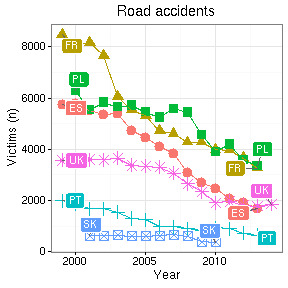
\includegraphics{2015-manu-roadacc-1}
\end{center}
\caption{Timeline indicating the number of people killed in road accidents in various countries based on data retrieved with the \CRANpkg{eurostat} package.}
\label{fig:transport}
\end{figure}




\section{Utilities}

\begin{table}[ht!]
\centering
\begin{tabular}{rllrr}
\toprule
  \hline
  & sex & geo & time & values \\ 
  \hline
  1 & T & AT & 1999.00 & 1079.00 \\ 
  2 & T & BE & 1999.00 & 1397.00 \\ 
  3 & T & BG & 1999.00 &  \\ 
  4 & T & CH & 1999.00 &  \\ 
  5 & T & CY & 1999.00 &  \\ 
  6 & T & CZ & 1999.00 & 1455.00 \\ 
   \hline
\bottomrule      
\end{tabular}
\caption{First lines of output from the \code{get\_eurostat()} function with the road accident data set identifier 'tsdtr420'.}
\label{tab:getdatatable}
\end{table}


\begin{table}[hb!]
\centering
\begin{tabular}{rllrr}
\toprule
  \hline
  & sex & geo & time & values \\ 
  \hline
  1 & Total & Austria & 1999.00 & 1079.00 \\ 
  2 & Total & Belgium & 1999.00 & 1397.00 \\ 
  3 & Total & Bulgaria & 1999.00 &  \\ 
  4 & Total & Switzerland & 1999.00 &  \\ 
  5 & Total & Cyprus & 1999.00 &  \\ 
  6 & Total & Czech Republic & 1999.00 & 1455.00 \\ 
   \hline
\bottomrule   
\end{tabular}
\caption{The output from \code{get\_eurostat()} (Table~\ref{tab:getdatatable}), now converted into human-readable labels by \code{label\_eurostat()}.}
\label{tab:getdatatable2}
\end{table}

Many entries in Table~\ref{tab:getdatatable} are not readily
interpretable, but a simple call \code{label\_eurostat(dat)} converts
the original identifier codes into human-readable labels (shown in
Table~\ref{tab:getdatatable2}) based on translations in the Eurostat
database. Labels are available in English, France and Germany.

The downloaded data sets are stored in cache by default to avoid
repeated downloads of identical data sets. This can speed up the
analysis. Storing an exact copy of the retrieved raw data on the hard
disk supports also the reproducibility when the source database is
constantly updated.

The Eurostat database includes a variety of demographic and health
indicators. We see, for instance, that overweight varies remarkably
across different age groups quantified by the body-mass index (BMI)
(Figure~\ref{fig:bmi} A). Sometimes the data from the eurostat
database requires more complex pre-processing. Let's consider a
question about distribution of sources of renewable energy in
different European countries. In order to summarise such sources one
needs to first aggregate all possible sources into a smaller number of
interesting groups. Then with the use of packages like \CRANpkg{dplyr}
or \CRANpkg{tidyr} one can process data, chop country names, filter
countries depending on production levels, normalize the within country
production. After a series of such transformations (see Appendix for
the source code) we can finally plot the data to discover that
countries vary a lot in terms of sources of renewable energy
(Figure~\ref{fig:bmi} B). Three-dimensional data sets such as this can
be conveniently visualized as triangular maps by using
the \CRANpkg{plotrix} \citep{plotrix} package.


\begin{figure}
\setkeys{Gin}{width=0.5\textwidth}
\begin{center}
\begin{tabular}{cc}
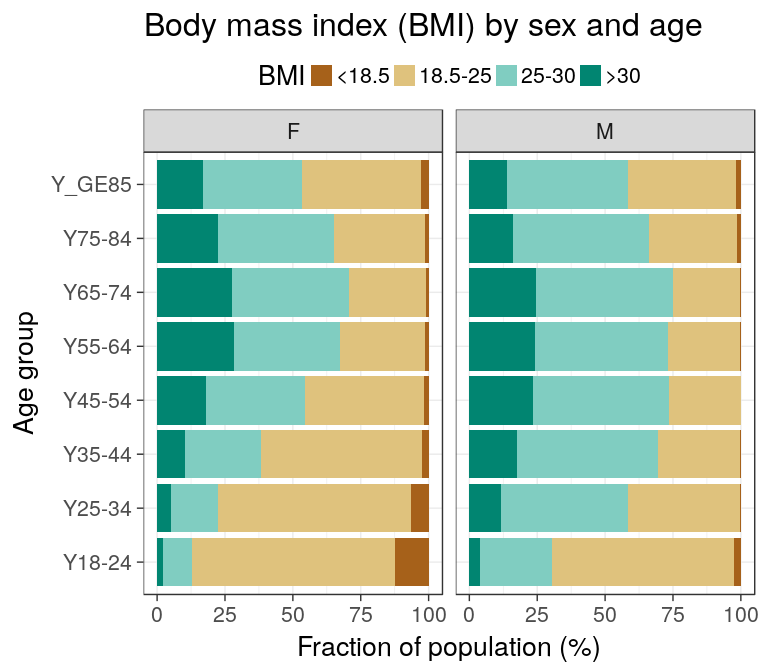
\includegraphics{2015-manu-bmi-1}
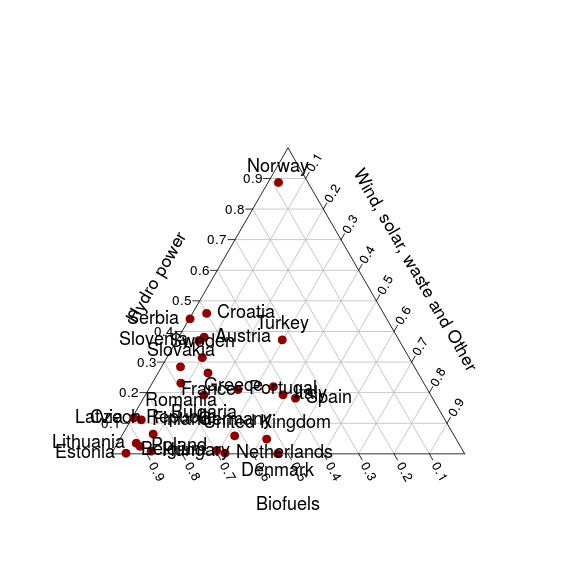
\includegraphics{2015-manu-energy-1}
\end{tabular}
\end{center}
\caption{{\bf A} The body-mass index in different age groups in Poland based on Eurostat table 'hlth\_ehis\_de1'. {\bf B} Distribution of sources of renewable energy production based on Eurostat table \texttt{ten00081}, year 2013. See the Appendix for the source code for both figures.}
\label{fig:bmi}
\end{figure}



\section{Geospatial information}

\subsection{Map visualizations}

The indicators in the Eurostat open data service are typically
available as annual time series grouped by country, and sometimes at
more refined temporal or geographic levels. Eurostat provides
complementary geospatial data on the corresponding administrative
statistical units to support visualizations at the appropriate
geographic resolution. The geospatial data sets are available as
standard
shapefiles\footnote{http://ec.europa.eu/eurostat/web/gisco/geodata/reference-data/administrative-units-statistical-units}. As
an example, let us look at disposable income of private households
(data set identifier
tgs00026\footnote{http://ec.europa.eu/eurostat/en/web/products-datasets/-/TGS00026}). This
information is provided at the geographic level of NUTS2 regions. This
is the intermediate level of territorial units in the Eurostat
regional classifications, and roughly corresponds to provinces or
states in each
country\footnote{http://ec.europa.eu/eurostat/web/nuts/overview}
(Figure~\ref{fig:mapexample}). The
example demonstrates how the Eurostat data sets and geospatial data,
retrieved with the eurostat package, can be combined with additional
visualization tools and other utilities including
\CRANpkg{grid} \citep{grid}, \CRANpkg{maptools} \citep{maptools}, \CRANpkg{rgdal} \citep{rgdal},
\CRANpkg{rgeos} \citep{rgeos}, \CRANpkg{scales} \citep{scales}, and
\CRANpkg{stringr} \citep{stringr}.

\begin{figure}
\setkeys{Gin}{width=0.7\textwidth}
\begin{center}
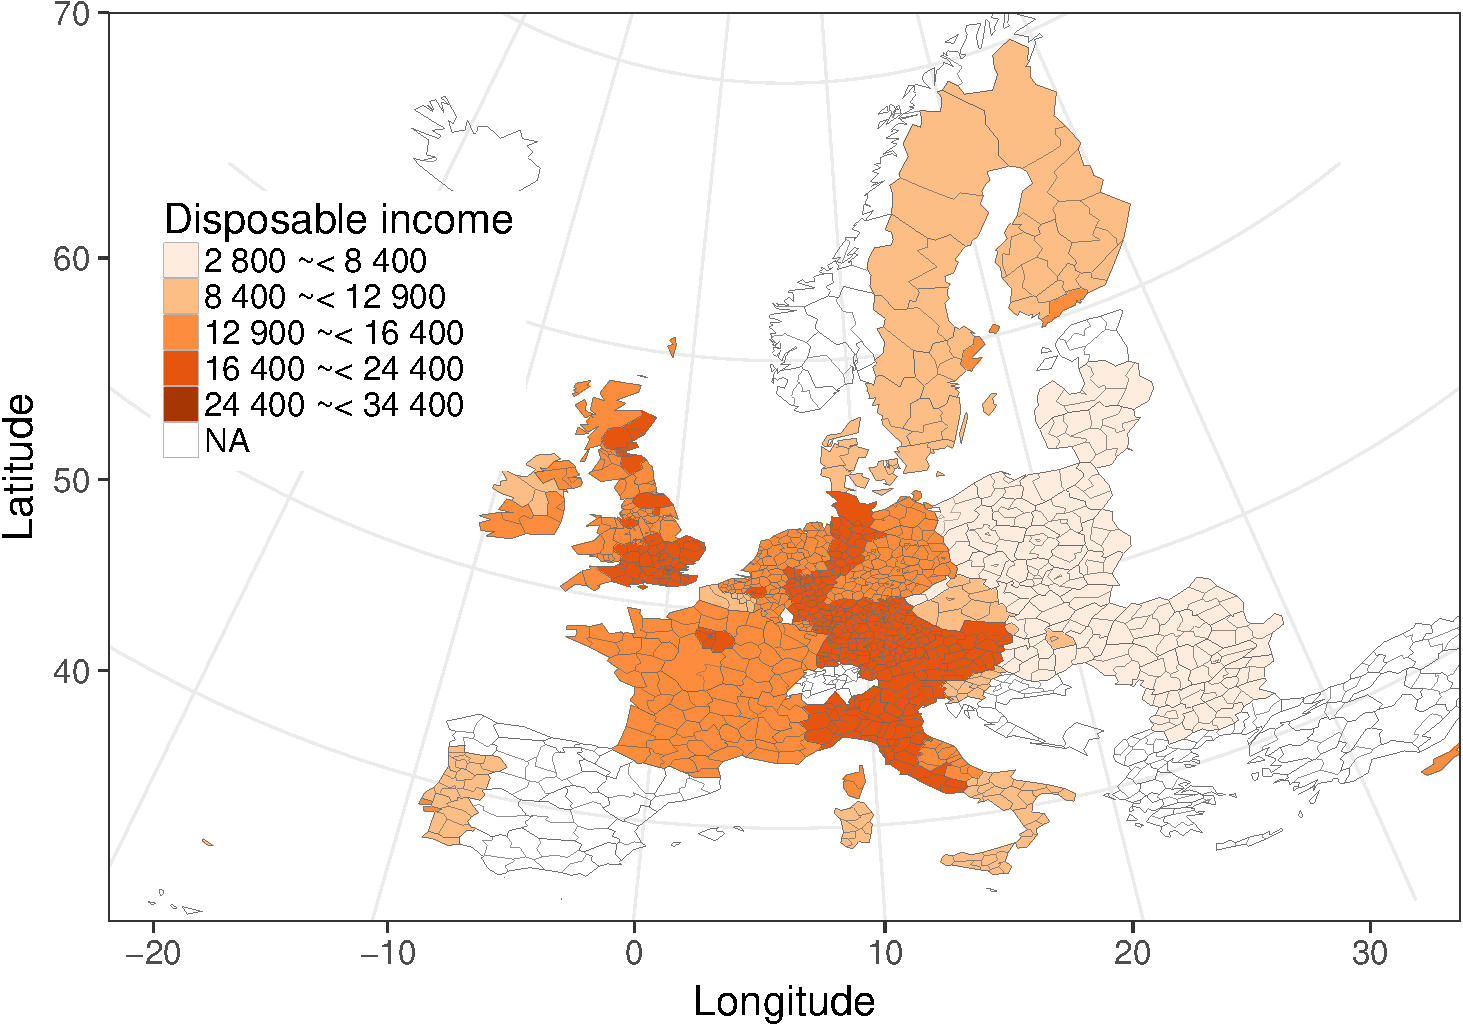
\includegraphics{2015-manu-mapexample-1}
\caption{Disposable income of private households across NUTS2-level national regions in European countries visualized based on geospatial data available from Eurostat.}
\label{fig:mapexample}
\end{center}
\end{figure}


\subsection{Default country groupings}

To facilitate further analysis and visualization of standard European
country groups, we have included ready-made country code lists. The
list of EFTA countries is retrieved, for instance, with:

\begin{example}
data(efta_countries)
\end{example}


This provides the EFTA country listing in
Table~\ref{tab:efta}. Similar lists are available for Euro area
(ea\_countries), EU (eu\_countries) and the EU candidate countries
(candidate\_countries). These auxiliary data sets facilitate the
selection of specific country groups in the analysis. The full name
and a two-letter identifier are provided for each country as provided
by the Eurostat database. The country codes follow the ISO 3166-1
alpha-2 standard, except that GB and GR are replaced by UK (United
Kingdom) and EL (Greece) in the Eurostat database,
respectively. Linking these country codes with external data sets can
be facilitated by conversions between different country coding
standards with the \CRANpkg{countrycode} package \citep{countrycode}.

\begin{table}[b]
\centering
\begin{tabular}{rll}
\toprule
  \hline
  & code & name \\ 
  \hline
  1 & IS & Iceland \\ 
  2 & LI & Liechtenstein \\ 
  3 & NO & Norway \\ 
  4 & CH & Switzerland \\ 
   \hline
\bottomrule   
\end{tabular}
\caption{The EFTA country listing from the eurostat R package.}
\label{tab:efta}
\end{table}




\section{Summary}

The \CRANpkg{eurostat} R package provides convenient tools to access open data
from Eurostat. Combining programmatic access to the data sets with
further analysis and visualization tools allows a seamless and
reproducible automation of the complete data analytical workflow from
accessing the raw data to statistical analysis and final
publication. The source code and installation instructions for the
latest development version of the eurostat package are available at
the github site, as well as the full source code of the figures and
tables of this manuscript\footnote{https://github.com/rOpenGov/eurostat},
where the Rmarkdown document provides reproducible documentation with
full algorithmic details on the analyses, and can be updated when new
versions of the Eurostat data become available.

The eurostat package provides one example of automated data retrieval
from institutional data repositories, featuring options such as
search, subsetting and cache. Possible future extensions and
improvements include implementation of specific data representation
formats to harmonize the data representation across similar data
sources and to facilitate subsequent tool development. In particular,
we should take further advantage of the existing spatiotemporal data
structures available in R, such as those provided by
the \CRANpkg{spacetime} package \citep{spacetime}, and construct
wrapper functions to speed up routine operations such as visualizing
the temporal and geospatial data sets from Eurostat. The package
source code can be freely used, modified and distributed under the
BSD-2-clause (modified FreeBSD) license. We welcome issues, bug
reports and other feedback.


\section*{Acknowledgements}

We are grateful to Eurostat for maintaining the open data service and
the rOpenGov\footnote{https://github.ropengov.io} for supporting R
package development. This work has been partially funded by Academy of
Finland (decision 293316). We also wish to thank Juuso Parkkinen and
Joona Lehtom{\"a}ki for feedback.


\bibliography{lahti-huovari-kainu-biecek}

\address{Leo Lahti\\
  Department of Mathematics and Statistics\\
  PO Box 20014 University of Turku\\
  Finland\\}
\email{leo.lahti@iki.fi}

\address{Janne Huovari\\
  Pellervo Economic Research PTT\\
  Eerikinkatu 28 A 00180 Helsinki\\
  Finland\\}
\email{janne.huovari@ptt.fi}

\address{Markus Kainu\\
  Research Department, The Social Insurance Institution of Finland\\
  PO Box 450, 00101 Helsinki\\
  Finland\\}
\email{markus.kainu@kela.fi}

\address{Przemyslaw Biecek\\
  Faculty of Mathematics, Informatics, and Mechanics\\
  University of Warsaw\\
  Banacha 2, 02-097 Warsaw\\
  Poland\\}
\email{P.Biecek@mimuw.edu.pl}

\newpage

\section{Appendix}

Source code for the obesity example (Figure~\ref{fig:bmi} A):

\begin{example}
library(dplyr)
tmp1 <- get_eurostat("hlth_ehis_de1", time_format = "raw")
tmp1 %>%
  dplyr::filter( isced97 == "TOTAL" ,
          sex != "T",
          age != "TOTAL", geo == "PL") %>%
  mutate(BMI = factor(bmi, 
                      levels=c("LT18P5","18P5-25","25-30","GE30"), 
                      labels=c("<18.5", "18.5-25", "25-30",">30"))) %>%
  arrange(BMI) %>%
  ggplot(aes(y=values, x=age, fill=BMI)) +
  geom_bar(stat="identity") +
  facet_wrap(~sex) + coord_flip() +
  theme(legend.position="top") + ggtitle("Body mass index (BMI) by sex and age")+xlab("\% of population")+scale_fill_brewer(type = "div")
\end{example}


Source code for the renewable energy example (Figure~\ref{fig:bmi} B):

\begin{example}
# All sources of renewable energy are to be grouped into three sets
> dict <- c("Solid biofuels (excluding charcoal)" = "Biofuels",
+          "Biogasoline" = "Biofuels",
+          "Other liquid biofuels" = "Biofuels",
+          "Biodiesels" = "Biofuels",
+          "Biogas" = "Biofuels",
+          "Hydro power" = "Hydro power",
+          "Tide, Wave and Ocean" = "Hydro power",
+          "Solar thermal" = "Wind, solar, waste and Other",
+          "Geothermal Energy" = "Wind, solar, waste and Other",
+          "Solar photovoltaic" = "Wind, solar, waste and Other",
+          "Municipal waste (renewable)" = "Wind, solar, waste and Other",
+          "Wind power" = "Wind, solar, waste and Other",
+          "Bio jet kerosene" = "Wind, solar, waste and Other")
# Some cleaning of the data is required
> energy3 <- get_eurostat("ten00081") %>%
+  label_eurostat(dat) %>% 
+  filter(time == "2013-01-01",
+         product != "Renewable energies") %>%
+  mutate(nproduct = dict[as.character(product)], # just three categories
+         geo = gsub(geo, pattern=" \\(.*", replacement="")) %>%
+  select(nproduct, geo, values) %>% 
+  group_by(nproduct, geo) %>%
+  summarise(svalue = sum(values)) %>%
+  group_by(geo) %>%
+  mutate(tvalue = sum(svalue),
+         svalue = svalue/sum(svalue)) %>%
+  filter(tvalue > 1000,
+         !grepl(geo, pattern="^Euro")) %>% # only large countrie
+  spread(nproduct, svalue)
# Triangle plot
> library(plotrix)
> par(cex=0.75)
> plotrix::triax.plot(as.matrix(energy3[, c(3,5,4)]),
+                      show.grid = TRUE,
+                      label.points = TRUE, point.labels = energy3$geo,
+                      pch = 19)
\end{example}


